\section{Introduction}
\label{sec:introduction}

Multimodal retrieval over egocentric video presents challenges unlike those in web image search or broadcast video retrieval. In lifelogging corpora, activities are observed from a first-person perspective, queried objects may be small or partially occluded, and speech transcripts are generated by automatic speech recognition systems that do not always align with the visual evidence available in a single frame. As a result, sparse keyword matching alone is often insufficient, particularly for visually grounded queries where the relevant signal is weak or absent in the transcript stream. These characteristics motivate retrieval architectures that treat dense visual representations as a primary signal rather than as a secondary reranking feature \cite{gurrin2024castle}.

The CASTLE 2024 dataset provides a realistic testbed for studying this problem. It contains 416,542 keyframes sampled at 5-second intervals across four recording days, spanning ten egocentric member cameras and five fixed room cameras: kitchen, living1, living2, meeting, and reading. Each frame follows the \textbf{HH\_NNNN.webp} naming convention, where \textbf{HH} denotes the hour of day and \textbf{NNNN} is a four-digit frame counter within that hour. Machine-generated ASR transcripts are aligned to frames using a 20-second sliding window, producing 145,140 transcript-frame pairs that supply conversational context when it is available.

Our system is organised as a three-stage pipeline consisting of feature extraction, multi-index retrieval, and final ranking. Approach A uses BM25 as a sparse text baseline over transcripts and \textbf{Florence-2} machine-generated visual captions, explicitly satisfying the assignment requirement for an inverted index while providing a transparent lexical baseline \cite{robertson2009probabilistic}. Approach B uses \textbf{SigLIP2} SO400M embeddings as the dense visual retrieval backbone, leveraging the strong cross-modal alignment induced by sigmoid-loss pre-training \cite{zhai2023sigmoid}. Approach C is the principal contribution. It combines BM25 scores, \textbf{BGE-large-en-v1.5} dense text embeddings, and \textbf{SigLIP2} visual embeddings through weighted late fusion, then applies cross-encoder reranking with the \textbf{bge-reranker-v2-m3} model over the top-50 candidates. This design allows the system to exploit complementary evidence from sparse lexical matching, dense semantic text retrieval, and dense visual similarity, while still preserving a controllable ranking pipeline \cite{chen2024bge}. Figure~\ref{fig:architecture} illustrates the seven-layer system architecture.

\begin{figure}[t]
  \centering
  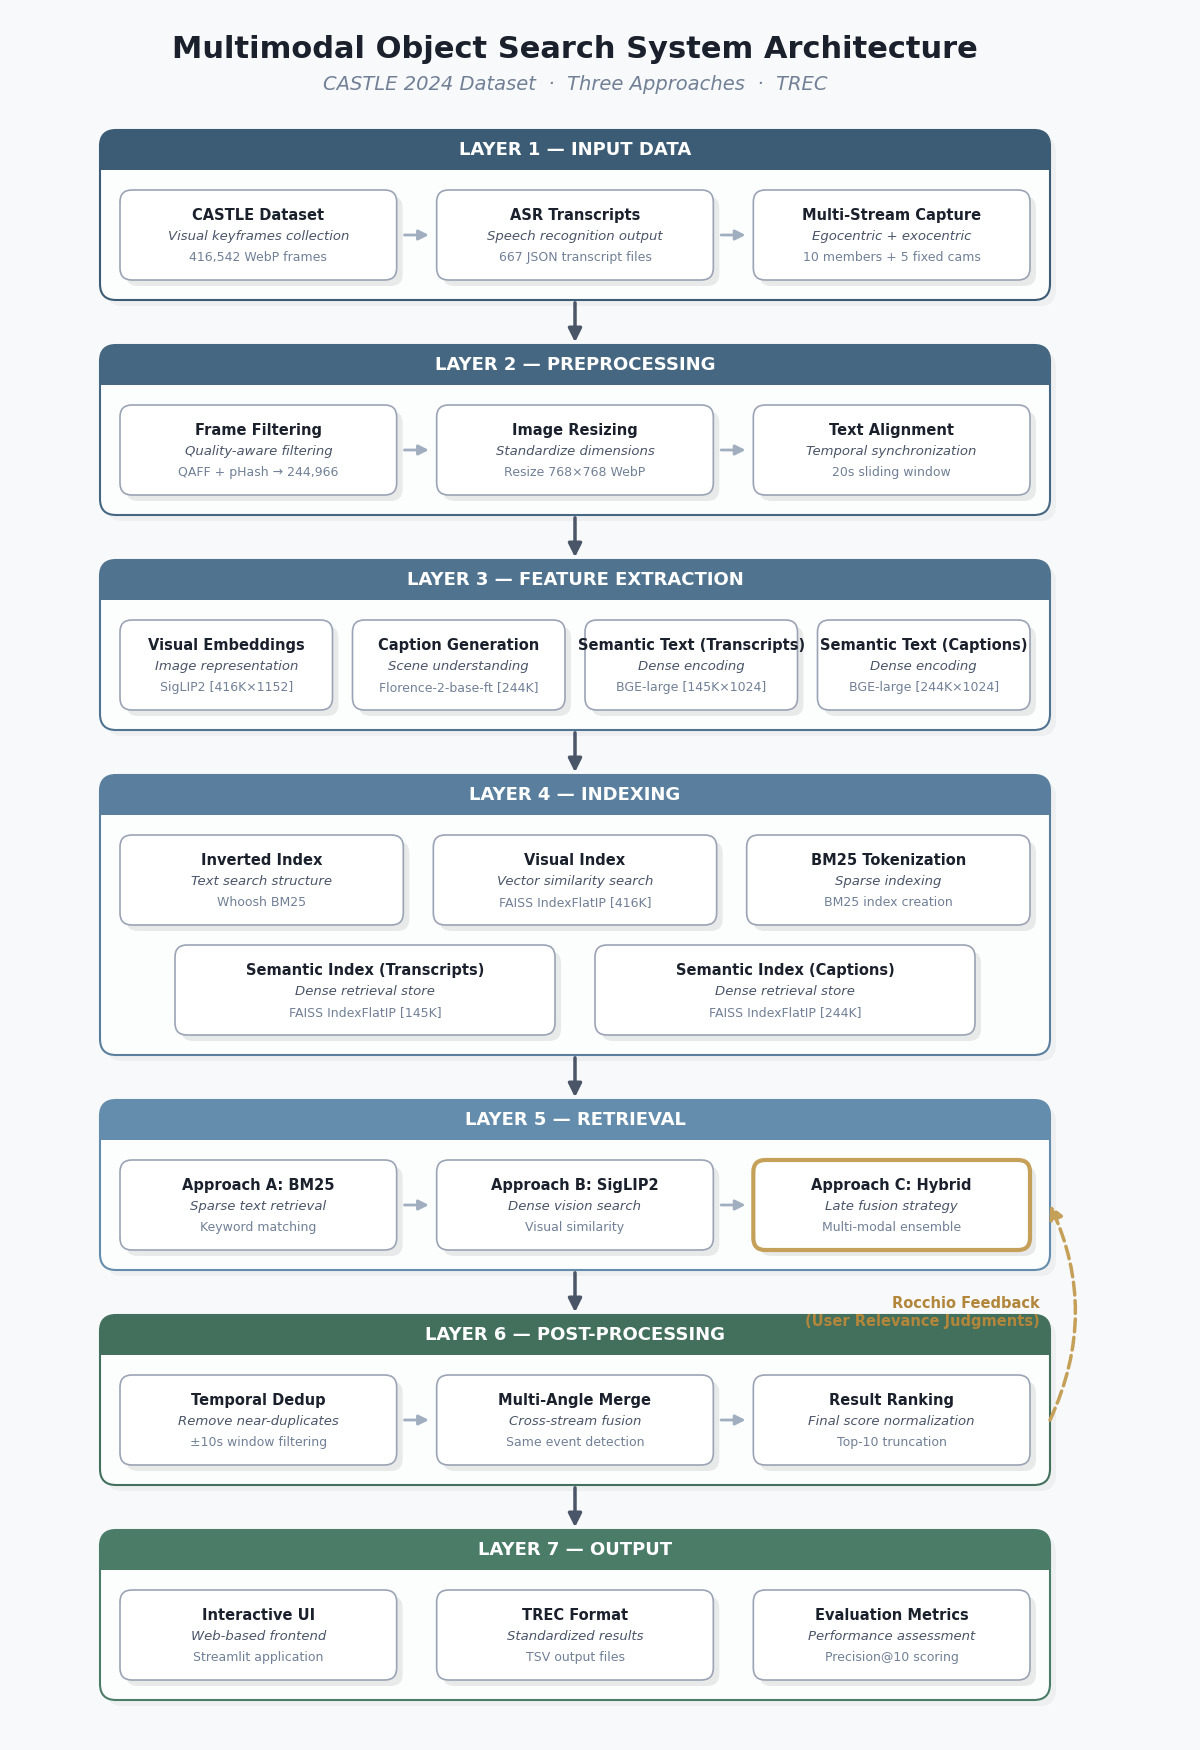
\includegraphics[width=\linewidth]{figures/architecture_diagram_v2}
  \caption{System architecture of the MOS pipeline. Seven layers cover input data, preprocessing, feature extraction, indexing, retrieval, post-processing, and output.}
  \label{fig:architecture}
  \Description{Seven-layer system diagram showing data input, preprocessing, feature extraction, indexing, retrieval, post-processing, and output stages in the MOS pipeline.}
\end{figure}

To support interactive exploration, we also provide a Streamlit interface with query selection, approach switching, result inspection, and Rocchio-style relevance feedback driven by \textbf{SigLIP2} vector blending \cite{rocchio1971relevance}. The remainder of the paper is structured as follows. Section~\ref{sec:indexing} describes the indexing pipeline, including the OCR hallucination gate. Section~\ref{sec:ranking} details the three retrieval approaches and post-processing stages. Section~\ref{sec:evaluation} presents the Precision@10 evaluation and analysis. Section~\ref{sec:conclusions} concludes the paper and outlines future work.
